不必要的对象复制可能是C++的低效之处。主要原因是这样做很简单,但很难关注到。看一下以下代码:

\begin{lstlisting}[style=styleCXX]
std::vector<int> v = make_v(… some args …);
do_work(v);
\end{lstlisting}

这个程序中,\texttt{v}被复制了多少次?答案取决于\texttt{make\_v()}和\texttt{do\_work()}函数的实现以及编译器的优化。这个例子涵盖了要讨论的一些语言细节。

\subsubsubsection{9.3.1\hspace{0.2cm}复制和参数传递}

我们将从第二个函数\texttt{do\_work()}开始。若函数以引用(\texttt{const}或非\texttt{const}形式)传递实参,则不进行复制。

\begin{lstlisting}[style=styleCXX]
void do_work(std::vector<int>& vr) {
	… vr is a reference to v …
}
\end{lstlisting}

若函数使用按值传递,则必须进行复制:

\begin{lstlisting}[style=styleCXX]
void do_work(std::vector<int> vc) {
	… vc is a copy of v …
}
\end{lstlisting}

如果\texttt{vector}对象很大,则复制\texttt{vector}对象的操作代价很高。必须复制\texttt{vector}对象中的所有数据,这是一个代价很高的函数调用。如果不需要\texttt{vector}的副本,那这里的复制就非常的低效。例如,如果只需要计算\texttt{vector}中所有元素的和(或其他计算),则不需要副本。乍一看,调用本身并没有告诉我们是否复制,但它应该是这样的。复制的决定属于函数的实现者,只有在考虑了需求和算法的选择后才能做出。对于前面提到的累加所有元素和的问题,正确的决定显然是通过(\texttt{const})引用传递\texttt{vector}对象,如下所示:

\begin{lstlisting}[style=styleCXX]
void do_work(const std::vector<int>& v) {
	int sum = 0;
	for (int x: v) sum += x;
	… use sum … 
}
\end{lstlisting}

使用值传递明显是低效的,并可能会认为是一个Bug,但是这种情况发生的频率比还挺高。特别是在模板代码中,作者只考虑了小型、轻量级的数据类型,但代码最终得到了比预期更广泛的使用。

另一方面,如果需要创建实参的副本,作为满足函数要求的一部分,使用参数传递是一种很好的方法:

\begin{lstlisting}[style=styleCXX]
	void do_work(std::vector<int> vc) {
		… vc is a copy of v …
	}
\end{lstlisting}

进一步处理数据之前,需要对数据应用一个所谓的固定环。假设多次读取固定位的值,每次访问都调用\texttt{std::min()}可能比创建结果的缓存副本的效率要低。也可以显式的制作一个副本,这可能会更有效,但这种优化不应该只是猜测,需要通过一个基准测试才能明确回答。

C++11引入了移动语义来解决部分不必要的复制。本例中,如果函数实参是右值,可以以任何方式使用,包括修改它(调用者在调用完成后无法访问该对象)。利用移动语义的常用方法是使用右值引用版本重载函数:

\begin{lstlisting}[style=styleCXX]
void do_work(std::vector<int>&& v) {
	… can alter v data … 
}
\end{lstlisting}

但是,如果对象本身支持移动,简单的值传递版本就有了亮点。参考以下代码:

\begin{lstlisting}[style=styleCXX]
void do_work(std::vector<int> v) {
	… use v destructively … 
}
std::vector<int> v1(…);
do_work(v1);                 // Local copy is made
do_work(std::vector<int>(…));    // rvalue
\end{lstlisting}

\texttt{do\_work()}的第一次调用使用了左值参数,因此在函数内部进行了局部复制(参数通过值传递!)。第二个调用使用右值或未命名的临时函数,由于\texttt{vector}有一个移动构造函数,函数的实参移动(而不是复制!)到形参中,移动\texttt{vector的}速度非常快。现在,在没有重载的情况下,通过函数实现,可以有效地处理右值和左值参数,现在已经看到了两个极端的例子。第一种情况下,不需要副本,显式的构造一份是低效的。第二种情况下,复制是一种合理的实现。正如即将看到的,并不是每一种情况都属于这些极端情况。

\subsubsubsection{9.3.2\hspace{0.2cm}使用复制进行实现}

还有一种中间情况,即选择的实现需要参数的副本,但实现本身并不是最优的。考虑下面的函数,需要按顺序输出:

\hspace*{\fill} \\ %插入空行
\noindent
\textbf{01\_vector\_sort.C}
\begin{lstlisting}[style=styleCXX]
void print_sorted(std::vector<int> v) {
	std::sort(v.begin(), v.end());
	for (int x: v) std::cout << x << “\n”;
}
\end{lstlisting}

对于整数\texttt{vector},这可能是最好的方法,对容器本身进行排序并按顺序打印。因为不应该修改原始容器,所以需要一个副本,而且需要利用编译器来创建一个副本也没有什么错。

但是如果\texttt{vector}的元素不是整数,而是一些大型对象呢?在这种情况下,复制\texttt{vector}就需要占用大量内存,而对其进行排序需要花费大量时间来复制大型对象。这种情况下,更好的实现可能是在不移动原始对象的情况下,创建指针\texttt{vector}并对其排序:

\hspace*{\fill} \\ %插入空行
\noindent
\textbf{01\_vector\_sort.C}
\begin{lstlisting}[style=styleCXX]
template <typename T>
void print_sorted(const std::vector<T>& v) {
	std::vector<const T*> vp; vp.reserve(v.size());
	for (const T& x: v) vp.push_back(&x);
	std::sort(vp.begin(), vp.end(), 
		[](const T* a, const T* b) { return *a < *b;});
	for (const T* x: vp) std::cout << *x << “\n”;
}
\end{lstlisting}

因为现在已经学会了\textit{永远不要猜测性能},所以直觉需要通过基准测试来确认。因为对已经排序的\texttt{vector}进行排序不需要任何复制,所以希望在基准测试的每次迭代中都有一个新的、未排序的\texttt{vector},如下所示:

\hspace*{\fill} \\ %插入空行
\noindent
\textbf{01\_vector\_sort.C}
\begin{lstlisting}[style=styleCXX]
void BM_sort(benchmark::State& state) {
	const size_t N = state.range(0);
	std::vector<int> v0(N); for (int& x: v0) x = rand();
	std::vector<int> v(N);
	for (auto _ : state) {
		v = v0;
		print_sorted(v);
	}
	state.SetItemsProcessed(state.iterations()*N);
}
\end{lstlisting}

当然,应该禁用打印,因为对I/O基准测试不感兴趣。另一方面,应该在不进行排序的情况下对复制\texttt{vector}进行基准测试,这样就可以知道所测量的时间的哪一部分花在了准备测试上。

基准测试确认,对于整数,复制整个\texttt{vector}对象并对其进行排序会更快:

%\hspace*{\fill} \\ %插入空行
\begin{center}
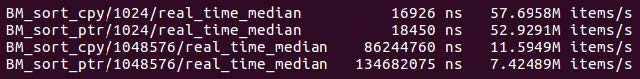
\includegraphics[width=0.9\textwidth]{content/3/chapter9/images/1.jpg}\\
图9.1 - 对整数\texttt{vector}排序的基准测试:复制方式和指针方式(间接)的对比
\end{center}

请注意,如果数组很小,而且所有数据都适合底层缓存,那么无论哪种方式,处理速度都非常快,而且速度差异很小。如果对象比较大,复制的代价也比较高,那么间接性方式就会比较高效:

%\hspace*{\fill} \\ %插入空行
\begin{center}
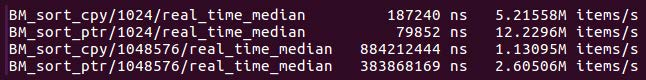
\includegraphics[width=0.9\textwidth]{content/3/chapter9/images/2.jpg}\\
图9.2 - 大型对象的\texttt{vector}排序基准测试:复制方式和指针(间接)方式
\end{center}

还有一种特殊情况,即实现时需要复制对象。

\subsubsubsection{9.3.3\hspace{0.2cm}复制存储数据}

C++中会遇到另一种数据复制的特殊情况。这种情况最常发生在类构造函数中,在类构造函数中,对象必须存储数据的副本,因此必须创建一个生命周期超过构造函数调用生命周期的副本。看一下这个例子:

\begin{lstlisting}[style=styleCXX]
class C {
	std::vector<int> v_;
	C(std::vector<int> ??? v) { … v_ is a copy of v … }
};
\end{lstlisting}

这里的目的是复制一份,低效率的做法是复制多个中间副本或一个不必要的副本。实现的标准方法是通过\texttt{const}引用获取对象,并在类内部复制:

\begin{lstlisting}[style=styleCXX]
class C {
	std::vector<int> v_;
	C(const std::vector<int>& v) : v_(v) { … }
};
\end{lstlisting}

如果构造函数的实参是左值,这是最高效的。但是,如果实参是右值(临时值),可以将它移到类中,从而不进行复制。这需要重载构造函数:

\begin{lstlisting}[style=styleCXX]
class C {
	std::vector<int> v_;
	C(std::vector<int>&& v) : v_(std::move(v)) { … }
};
\end{lstlisting}

缺点是需要编写两个构造函数,但如果构造函数有几个参数,并且每个参数都需要复制或移动,情况就麻烦了。按照这种模式,将需要6个构造函数重载来处理3个参数。

另一种方法是按值传递所有参数,并移动参数。看下代码:

\begin{lstlisting}[style=styleCXX]
class C {
	std::vector<int> v_;
	C(std::vector<int> v) : v_(std::move(v)) 
	{ … do not use v here!!! … }
};
\end{lstlisting}

形参\texttt{v}现在是一个处于已移动状态的对象,不应该在构造函数体中再使用。如果实参是左值,则创建一个副本来构造形参\texttt{v},然后移动到类中。如果实参是右值,则将其移动到形参\texttt{v}中,然后再次移动到类中。如果移动成本较低,这种模式就很高效。然而,如果对象的移动代价很高,或者根本没有移动构造函数(只能复制),最终则会进行两次复制,而不是一次。 

我们关注的是将数据放入函数和对象的问题。但是当需要返回结果时,复制也可能发生。这里的考虑因素完全不同,需要分别研究。

\subsubsubsection{9.3.4\hspace{0.2cm}复制返回值}

本节开头的示例包含了这两种类型的复制。特别是这一行:

\begin{lstlisting}[style=styleCXX]
std::vector<int> v = make_v(… some args …);
\end{lstlisting}

生成的\texttt{v}是由\texttt{make\_v}函数返回的:

\hspace*{\fill} \\ %插入空行
\noindent
\textbf{02\_rvo.C}
\begin{lstlisting}[style=styleCXX]
std::vector<int> make_v(… some args …) {
	std::vector<int> vtmp;
	… add data to vtmp …
	return vtmp;
}
\end{lstlisting}

理论上,这里可以进行不止一次的复制:局部变量\texttt{vtmp}复制到\texttt{make\_v}函数的(未命名)返回值中,又复制到最终结果\texttt{v}中。首先,\texttt{make\_v}的临时返回值会移动,而不是复制到\texttt{v}中。但即使是这样,也可能不会发生。如果用自己的类,而不是\texttt{std::vector}来尝试这段代码,会看到这里既没有使用复制构造函数,也没有使用移动构造函数:

\hspace*{\fill} \\ %插入空行
\noindent
\textbf{02\_rvo.C}
\begin{lstlisting}[style=styleCXX]
class C {
	int i_ = 0;
	public:
	explicit C(int i) : i_(i) { 
		std::cout << “C() @” << this << std::endl;
	}
	C(const C& c) : i_(c.i_) {
		std::cout << “C(const C&) @” << this << std::endl;
	}
	C(C&& c) : i_(c.i_) {
		std::cout << “C(C&&) @” << this << std::endl;
	}
	~C() { cout << “~C() @” << this << endl; }
	friend std::ostream& operator<<( std::ostream& out,
	const C& c) {
		out << c.i_; return out;
	}
};  
C makeC(int i) { C ctmp(i); return ctmp; }
int main() {
	C c = makeC(42);
	cout << c << endl;
}
\end{lstlisting}

这个程序输出如下内容(对于大多数编译器,必须开启某种级别的优化):

%\hspace*{\fill} \\ %插入空行
\begin{center}
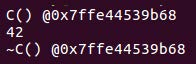
\includegraphics[width=0.4\textwidth]{content/3/chapter9/images/3.jpg}\\
图9.3 - 程序按值返回一个对象的输出
\end{center}

只构造和销毁了一个对象,这是编译器优化的结果。这里使用的优化为\textbf{返回值优化(RVO)},编译器认识到所涉及的三个对象——局部变量\texttt{ctmp}、未命名的临时返回值和最终结果\texttt{c}——都是相同的类型。此外,编写的代码都不可能同时观察到这两个变量。因此,在不改变可观察行为的情况下,编译器可以为这三个变量使用相同的内存位置。调用函数之前,编译器需要分配用于构造最终结果\texttt{c}的内存。这个内存地址由编译器传递到函数中,用于在相同的位置构造局部变量\texttt{ctmp}。因此,当函数\texttt{makeC}结束时,根本不需要返回任何东西,结果已经在它应该在的地方了。这就是RVO。

虽然RVO看起来很简单,但它有几个微妙之处。 

首先,这是一种优化。这意味着编译器通常不必这样做(如果编译器不这样做,可能需要一个更好的编译器),这是一种非常特殊的优化。通常,编译器可以对程序做任何事情,只要不改变可观察对象的行为。可观察行为包括输入、输出和访问易失性存储器。然而,这种优化导致了一个可观察的变化,复制构造函数和匹配的析构函数的预期输出不见了。实际上,这是一个例外:编译器允许消除复制或移动构造函数和相应的析构函数的调用,即使这些函数有包含可观察行为的副作用,并且这个例外不局限于RVO。通常,不能仅仅因为编写了一些似乎在进行复制的代码,就指望调用复制和移动构造函数。这就是所谓的\textbf{忽略复制}(或对于移动构造函数来说,就是\textbf{忽略移动})。

其次,(再次)这是一种优化。代码必须先编译,然后才能进行优化。如果对象没有任何复制或移动构造函数,这段代码将无法编译,所以将永远不会进入优化步骤,该步骤将删除所有对这些构造函数的调用。若在我们的例子中删除了所有的复制和移动构造函数,就很容易得到失败的结果:

\begin{lstlisting}[style=styleCXX]
class C {
	…
	C(const C& c) = delete;
	C(C&& c) = delete;
}; 
\end{lstlisting}

编译现在会失败,确切的错误信息取决于编译器和C++标准级别。在C++17中,看起来是这样的:

%\hspace*{\fill} \\ %插入空行
\begin{center}
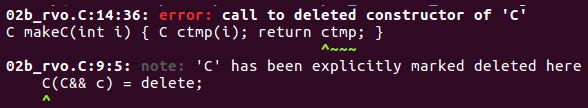
\includegraphics[width=0.9\textwidth]{content/3/chapter9/images/4.jpg}\\
图9.4 - 使用Clang(支持C++17或C++20)编译的输出
\end{center}

特殊情况是,即使删除了复制和移动操作,程序仍然可以编译。稍微修改一下\texttt{makeC}函数:

\begin{lstlisting}[style=styleCXX]
C makeC(int i) { return C(i); }
\end{lstlisting}

C++11和C++14没有什么变化。然而,在C++17及以上版本中,这段代码可以很好地编译。注意,与前一个版本的差别:返回的对象过去是左值,它有一个名称。现在它是一个右值,一个未命名的临时值。虽然\textbf{命名RVO(NRVO)}仍然是一种优化,但未命名RVO是强制性的,因为C++17不再认为其是一个忽略复制。该标准规定,一开始就不要求复制或移动。 

最后,可能想知道是否必须使用内联函数,以便编译器在编译函数本身时知道返回值在哪里。可以进行一个简单的测试,可以确信事实并非如此:即使函数\texttt{makeC}位于单独的编译单元中,RVO仍然会发生。因此,编译器必须将结果的地址发送到函数的调用点。如果不返回函数的结果,而是将结果的引用作为附加参数传递,开发者也可以做类似的事情。当然,必须首先构造该对象,而编译器生成的优化不需要额外的构造函数调用。 

可能会看到不依赖RVO的建议,但会强制执行返回值的移动:

\begin{lstlisting}[style=styleCXX]
C makeC(int i) { C c(i); return std::move(c); }
\end{lstlisting}

如果RVO没有发生,程序将承担复制操作的性能损失,而移动操作显然是更好的选择。然而,这种观点是错误的。要理解原因,请仔细查看图9.4中的错误消息:编译器报错说移动构造函数删除了,尽管\texttt{ctmp}是左值,并应该复制。这不是编译器的错误,但反映了标准所要求的行为。在返回值时进行优化是可能的,但编译器决定是否这么做取决于上下文,编译器必须首先找到一个移动构造函数来返回结果。如果没有找到移动构造函数,则执行第二次查找。这一次,编译器会寻找复制构造函数。在这两种情况下,编译器实际上是在执行重载解析,因为对象可以有许多复制或移动构造函数。因此,没有理由写一个显式的移动,编译器将自己生成一个。但这有什么不好的呢?其危害在于,使用显式移动将禁用RVO。需要一个移动,那么就获得一个。虽然移动可能只需要很少的工作,但RVO根本没有工作量,而且不工作总是比有工作快。

如果删除了移动构造函数,而没有删除复制构造函数,会发生什么?如果两个构造函数都删除了,编译仍然会失败。声明一个已删除的成员函数,与不声明任何成员函数是不同的。如果编译器对移动构造函数执行重载解析,将找到一个移动构造函数(即使这个构造函数被删除了)。编译失败的原因是,因为重载解析选择一个已删除的函数作为最佳(或唯一)重载。如果想强制使用复制构造函数(当然是以科研的名义),就不必声明任何移动构造函数。 

现在,已经看到了隐藏在代码中的复制对象,从而会有拉低程序性能的危险。能做些什么来避免无意的复制吗?我们稍后会给出一些建议,但先让我们回到已经使用过的一种方法:指针。

\subsubsubsection{9.3.5\hspace{0.2cm}使用指针避免复制}

传递对象时避免复制对象的一种方法是传递指针。如果不需要管理对象的生命周期,那这是最简单的方式。如果函数需要访问一个对象,但不需要删除它,那么通过引用或原始指针传递对象是最好的方式(在上下文中,引用实际上只是一个不能为空的指针)。 

类似地,可以使用指针从函数返回一个对象,但这需要注意一些问题。首先,对象必须在堆上分配。绝对不能返回指向局部变量的指针或引用。参考以下代码:

\begin{lstlisting}[style=styleCXX]
C& makeC(int i) { C c(i); return c; } // Never do this!
\end{lstlisting}

其次,调用者负责删除对象,因此函数的每个调用者都必须知道对象是如何构造的(\texttt{new}操作符不是构造对象的唯一方法,不过是最常见的方法而已)。这里的最佳解决方案是返回智能指针:

\hspace*{\fill} \\ %插入空行
\noindent
\textbf{03\_factory.C}
\begin{lstlisting}[style=styleCXX]
std::unique_ptr<C> makeC(int i) {
	return std::make_unique<C>(i);
}
\end{lstlisting}

注意,这样的工厂函数应该返回唯一指针,即使调用者可以使用共享指针来管理对象的生命周期:从唯一指针移动到共享指针很容易,成本也很低。

说到共享指针,它们通常用于传递生命期由智能指针管理的对象。除非目的是同时传递对象的所有权,否则这又是一个不必要和低效的复制的例子。复制共享指针开销也不小。若我们有一个由共享指针管理的对象,以及一个需要操作这个对象而不需要占有它的函数,应该怎么办呢?就可以使用原始指针:

\begin{lstlisting}[style=styleCXX]
void do_work1(C* c);
void do_work2(const C* c);
std::shared_ptr<C> p { new C(…) };
do_work1(&*p);
do_work2(&*p);
\end{lstlisting}

函数\texttt{do\_work1()}和\texttt{do\_work2()}的声明告诉我们开发者的意图,这两个函数都操作对象而不删除它。第一个函数修改对象,第二个则不然。这两个函数都希望在没有对象的情况下调用,并将处理这种特殊情况(否则,参数将通过引用传递)。 

类似地,只要对象的生命周期是在别处管理,就可以创建原始指针的容器。如果希望容器管理其元素的生命周期,但又不想将对象存储在容器中,可以则使用具有唯一指针的容器来完成这项工作。 

现在是时候给出一些通用的指导指南了,这些指导指南将帮助我们避免不必要的复制,以及相应的低效率。

\subsubsubsection{9.3.6\hspace{0.2cm}如何避免不必要的复制}

也许为了减少意外的、无意义的复制,可以做的事情是确保所有数据类型都是可移动的,如果实现移动比复制更廉价的话。如果有容器库或其他可重用代码,请确保支持移动。 

下一个建议有些笨拙,但可以节省大量调试时间:如果类型复制成本很高,那么就从一开始就让它不可复制,将复制和赋值操作声明为删除。如果类支持快速移动,则提供移动操作。当然,这将防止任何复制,无论是有意义还是无意义。希望有意义复制很少发生,可以实现一个特殊的成员函数,如\texttt{clone()},将创建对象的副本。至少这样,所有的复制在代码中是显式和可见的。如果类既不能复制也不能移动,就不能在STL容器中使用它,而包含唯一指针的容器是一种很好的替代方法。 

向函数传递参数时,尽可能使用引用或指针。如果函数需要复制实参,则考虑按值传递,并从实参移动。记住,这只适用于支持移动的类型,请参阅第一条准则。

关于传递函数参数的建议也可以应用于临时局部变量(毕竟,函数形参基本上就是函数作用域中的临时局部变量)。这些应该是可以参考的,除非需要复制。不过,这并不适用于整数或指针等内置类型,复制它们比间接访问要廉价。在模板代码中,无法知道类型是大是小,因此使用引用并依赖于编译器优化,可以避免不必要的(内置类型)间接访问。

当从函数返回值时,第一选择应该是依赖RVO和忽略复制。只有当发现编译器不执行这种优化,或这种优化对特定情况有影响时,才应该考虑其他方法。使用带有输出参数的函数和使用在动态分配的内存中构造结果,并返回智能指针(如\texttt{std::unique\_ptr})的工厂函数。 

最后,检查算法和实现,注意是否存在不必要的复制。恶意的复制和无意的复制对性能的影响是一样的。

我们已经解决了C++程序中影响效率的第一个问题,即对象的不必要复制。紧随其后的是糟糕的内存管理。














